\documentclass[10pt,letterpaper]{report}
\usepackage[utf8]{inputenc}
\usepackage{amsmath}
\usepackage{amsfonts}
\usepackage{amssymb}
\usepackage{graphicx}
\usepackage{textcomp}
\usepackage{mathtools}
\usepackage[left=2cm,right=2cm,top=2cm,bottom=2cm]{geometry}
\author{Brandon Caudell}
\title{Combinatorics of Rubik's Cubes}
\DeclarePairedDelimiter\ceil{\lceil}{\rceil}
\DeclarePairedDelimiter\floor{\lfloor}{\rfloor}
\begin{document}
\maketitle
\newpage 
\tableofcontents
\newpage 
\chapter{Introductory Information}
\section{Origins of the Rubik's Cube}
\section{Basic Terminology}
The standard 3x3 Rubik's Cube has six colors, one for each face.  The typical color scheme is white, yellow, red, orange, green, and blue.  The cube contains 26 external pieces, known as \textbf{cubies} or simply pieces.  These cubies come in 3 variants: \textbf{centers}, \textbf{edges}, and \textbf{corners}.  Center cubies contain only one colored sticker, edge pieces contain two stickers, and corner cubies contain three stickers.\\

Each of the cube's six faces can be independently rotated by multiples of 90\textdegree.  When held in a particular position, the six faces of the cube are generally regarded as front, back, left, right, up, and down.  These terms give rise to the standard move notation of F,B,L,R,U,D to denote clockwise rotations by 90\textdegree of each face.\\

These six moves are enough to scramble and solve the puzzle in any possible way, though it is convenient to define addition moves for clarity.  An apostrophe is used to denote a counter-clockwise move, so F' is a counter-clockwise rotation about the front face.  Adding a superscript 2 denotes performing a move twice, i.e. a 180\textdegree rotation, so $B^2$ is a 180\textdegree rotation of the back face.  This is regarded as a half-turn.  Note that by symmetry of the square faces, performing a clockwise move twice is equivalent to performing the counter-clockwise version twice, i.e. $L^2 \cong (L')^2$, so we just use the first notation.  Also note that repeating a clockwise-move (quarter-turn) three times is equivalent to a single counter-clockwise move, and vise versa.\\

Occasionally, it is useful to talk about \textbf{slice} moves.  These are moves obtained by rotating any of the three central "slices" of the cube.  In the standard 3x3 cube, these are denoted by lowercase variants of the same 6 letters, with apostrophes and exponents having the same meaning as before.  Note that if we talk about a slice relative to a particular face, that face still defines the direction of the rotation, but we actually rotate the cubies one layer "deeper" into the cube.  These slice moves are isomorphic at the cube level to performing two face turns on opposite faces, i.e. the slice move $r \cong R'L$ (rotating the right face counter-clockwise and the left face clockwise).  Although the two move sequences are isomorphic, they leave the cube as a whole oriented differently, hence why it is useful to define them even if they are rarely used in the 3x3 cube.  \\

We need to establish a convention in how to read these move sequences.  Since moves, in general, are not commutative, reading a sequence of moves such as $LFR$ from right-to-left or left-to-right changes the resulting cube.  While mathematically this sequence of moves is very similar to function composition, which is typically done right-to-left, it is easier for us to "read off" a move sequence left-to-right, so that is the convention that we will operate under.  In cases where a right-to-left order makes sense, we will formally declare that distinction. \\

Note that when applying face moves to a cube, the center cubies remain fixed.  The four edge and four corner pieces on a face will rotate around, but the centers always maintain the same orientation relative to each other.  This extends to slice moves as well (since slice moves can be attained by a composition of face turns), but note that in slice moves the centers may move on the cube as a whole.  Their relative orientations, however, always remain the same.  In the standard coloring, white is opposite yellow, red is opposite orange, blue is opposite green, and if white is held as the bottom face then blue is to the left of red.  Because of these fixed centers, when solving a cube, the solver always knows what color a face must end up.
\section{Larger Cubes}
Unsurprisingly, larger cubes present more options.  Not just in the number of permutations that can be obtained, but in the number of different cases one must handle when solving.  Thus, our notation and understanding must adapt to different cube sizes.  In this report, we denote the size of a cube as its \textbf{order}, i.e. an order-3 cube is the standard 3x3 one.  Note that larger cubes may have multiple center cubies, and they need not be at the centers of faces.  We still use this terminology, though. \\

For cubes of higher order, we gain additional move options.  Whereas on the standard cube, we only needed 6 moves to scramble and solve, we will need 3 more moves for each increase in order by 1.  A proof of this fact will be given later, but we will outline the notation here.  We still use capital letters to denote face moves, and these 6 moves will never change even as order increases.  As the size of the cube goes up, what will change is the number of distinct slice moves that can be performed.  For a cube of order $r$, there are $\floor{\frac{r}{2}}-1$ \textit{indecomposable} slice moves for each face.  By indecomposable, we mean moves not isomorphic to any other move sequences (so the slice moves in our 3x3 cube are decomposable and therefore less important).  For the standard cube, this gives that there are no indecomposable slice moves.  For the 4x4 cube (also known as the Rubik's Revenge), there is one slice move per face.\\

To denote which slice move we are talking about (as there may be many for large cubes), we use a subscript indexed from 1 to this $\floor{\frac{r}{2}}-1$.  In the case of the order-4 and 5 cubes, we may also use the lower-case letter variant as before, i.e. $r = R_1$.  Primes and powers still work as before.  While slightly clunky, this notation allows us to unambiguously denote which move is being performed. \\

One important consideration with larger cubes is the presence or absence of fixed centers.  As we showed, the 3x3 cube has center cubies that never change orientation.  This is true of all odd-order cubes, as the only moves that would move the centers at all can be decomposed into other moves that leave the centers untouched (possibly with a rotation of the cube as a whole in order to maintain directionality).  Even-order cubes, however, lose this nicety.  Since every move is unique and indecomposable, and there are multiple center cubies that will move independently of each other, it is up to the solver to ensure that the faces are actually reassembled in the correct relative orientations.  Not only must all colors be reassembled opposite their correct opposing color, but the relative orientations must be correct as well.  For instance, the white-red-blue corner piece is oriented such that the blue face should be left of red if the white face is pointed down.  If this orientation is not upheld, then the solve will not complete.
\chapter{Groups in the Rubik's Cube}
The first obvious question regarding the Rubik's Cube is ``How many possible scrambled states can the puzzle be in?''.  In order to answer this question, we need to understand the cube and its moves as an algebraic group.  We will start at a larger group and refine it down to our answer.
\section{The Sticker Group}
Given a cube of order $n$, it is easy to count the total number of stickers on it to be $6n^2$.  These stickers are partitioned into 6 different colors, one color per face on the solved cube.  Although clearly each sticker is ``locked'' to a cubie and thus the locations on the cube it can be moved to via legal moves are very limited, it is useful to think about what could happen if this constraint were removed. \\

If we were to take all the stickers off of the plastic cube body and rearrange them with no restrictions, then in how many ways could we do this?  If we assume each sticker is distinguishable (two red stickers can somehow be differentiated), then this sticker arrangement is just a permutation of $6n^2$ items.  We denote the algebraic group of these sticker rearrangements as the \textbf{Sticker Group of order n}.  The symbol we will use for this is $\mathcal{S}_n$.  This group is isomorphic to the symmetric group of order $6n^2$ for obvious reasons.  Thus, $\mathcal{S}_n \cong \mathfrak{S}_{6n^2}$. \\

Clearly, this is an extremely loose upper bound on the number of possible states of a valid Cube.  Let us go one level closer to the answer to our question.

\section{The Color Group}
As we mentioned, the Sticker Group makes the assumption that each sticker is distinguishable.  While this assumption is warranted in certain cases, from a solver's perspective, there really is no difference between different stickers of the same color, except in rare cases.  For instance, some 7x7 Cubes are ``pillowed'' such that the sides of the cube bulge out for various manufacturing and ergonomic reasons.  In this case, edge and corner stickers are different shapes to accommodate the shape of the (not really) cube.  This is a rare case, however, and generally we can regard the stickers of a color as being indistinguishable.\\

This gives rise to a smaller group of permutations of stickers subject to this indistinguishability.  We define a map $\pi : [6n^2] \rightarrow [6]$ where $[k] = \{1,2,...,k\}$.  The image of this map is the color set of the cube.  This map assigns each ``sticker index'' to its color, and evenly partitions the stickers into six color blocks each of size $n^2$.  We can use this map to partition the full group $\mathcal{S}_n$ into equivalence classes based on $\sigma_1 =_\pi \sigma_2 \iff (\pi \cdot \sigma_1) = (\pi \cdot \sigma_2)$ as functions, i.e. the color of the stickers at every location in the two stickerings  is the same. \\

Thus, we arrive at the quotient group $\mathcal{S}_n \slash \mathfrak{S}_{n^2}^6$.  The factor of this quotient group comes from the equivalence class of the identity in $\mathcal{S}_n$ -- the solved cube state.  We can permute any stickers within each of the 6 faces, and there are $n^2$ stickers in each.  We will refer to this quotient group as the \textbf{Color Group of order n}, denoted $\mathcal{C}_n \cong \mathcal{S}_n \slash \mathfrak{S}_{n^2}^6$. Its cardinality can be easily counted as \begin{align*}
|\mathcal{C}_n| &= [\mathcal{S}_n : \mathfrak{S}_{n^2}^6] \\
&= \frac{|\mathcal{S}_n|}{|\mathfrak{S}_{n^2}^6|} \\
&= \frac{(6n^2)!}{(n^2!)^6}
\end{align*}
which we know will be a positive integer by definition of index. \\

While still not very close to the Rubik's Group we desire, it is useful to consider this group because of the equivalence relation it is defined on.  When we talk about a ``solved state'' of a cube of order n, we currently have no guarantee of its uniqueness in $\mathcal{S}_n$.  While clearly there is a unique solved state in the basic 3-Cube (because all pieces are distinguishable by their stickers), this need not hold for larger cubes.  Since larger cubes have cubies that look that same (multiple centers per face, multiple edge cubies with the same two colors), we can imagine a case where a solver correctly solves the cube, returning each face to a solid color, but unknowingly swaps some indistinguishable pieces along the way.  While this cube state is not the identity in $\mathcal{S}_n$, it is the identity in $\mathcal{C}_n$. \\

We now turn our attention away from the stickers of the cube, and to the pieces themselves.  Since these are the items the solver interacts with, working with them is more likely to give us the number of states of the cube.

\section{The (Re)assembly Group}
Instead of moving the stickers around freely, what if we leave the stickers alone and move the pieces around the cube?  By that, I mean taking the cube apart and arbitrarily reassembling the cubies.  This number of possible reassemblies is certainly smaller than $|\mathcal{C}_n|$, but what is its size?  The calculation is slightly harder, but still not difficult. \\

Given a cube of order $n$, how many of each type of cubie are there?  Well, there will always be 8 corners.  There will always be 12 ``edge segments'' on the cube, each of which will contain $n-2$ pieces, so that gives us $12n - 24$ edge cubies.  For the center cubies (which, again, need not actually be at the centers of faces), there are 6 faces' worth, each having $(n-2)^2$.  So some algebra gives us that there are a total of $6(n^2  - 4n + 4) = 6n^2 - 24n + 24$ total center cubies. \\

So we know that the number of reassemblies will have as factors the possible permutations of these three types of cubies.  We also need to consider the fact that the edges and corners have multiple orientations per piece, though.  Each edge has 2 orientations, and each corner has 3.  From this information, we can calculate the number of possible cube reassemblies.  We will call this algrebraic group the \textbf{Assembly/Reassembly Group of order n}, and denote it by $\mathcal{A}_n$.  This group is clearly a subgroup of $\mathcal{S}_n$, though not necessarily of $\mathcal{C}_n$ as we are making no guarantees about indistinguishability of similar pieces.  We can calculate its cardinality as \begin{align*}
|\mathcal{A}_n| &= \frac{8! \cdot 3^8 \cdot (12n-24)! \cdot 2^{12n-24} \cdot (6n^2 - 24n + 24)!}{24} \\
&= 7! \cdot 3^7 \cdot (12n-24)! \cdot 2^{12n-24} \cdot (6n^2 - 24n + 24)!
\end{align*}
This calculation arises fairly obviously just from considering the number of each piece and our freedom to arrange them.  The division by 24 accounts for the fact that any given reassembly of the cube will be overcounted by a factor of 24 since we can rotate the cube freely in space in 24 orientations without really changing the assembly of the cubies.  In group theory, we can use this same information to arrive at a decomposition for $\mathcal{A}_n$ into subgroups for each piece type.  Since the arrangements of center, edge, and corner cubies are all independent, we can write a direct product
\begin{align*}
\mathcal{A}_n \cong
\mathcal{A}_n^C \times
\mathcal{A}_n^E \times
\mathcal{A}_n^R
\end{align*}
where the terms are the subgroups concerning assemblies of the centers, edges, and corners, respectively.  These subgroups are easier to work with.  The previous factor of 24 will be addressed in the subgroup of corners. \\

The subgroup of permutations of the centers is just a symmetric group of the appropriate size.  Since we don't need to worry about orientations of these stickers (as rotating a sticker by itself on a Cube has no significance), this group isomorphism is obvious. $ \mathcal{A}_n^C \cong \mathfrak{S}_{6n^2 - 24n + 24}$. \\

The subgroup of edges is slightly more complicated, but still not hard.  We have $12n-24$ edges that can be positioned freely, giving a symmetric group.  On top of that, we can also orient each edge in one of two ways.  Thus, each edge orientation is an element of $\mathbb{Z}_2$.  We can express the interaction of these two groups using either a semidirect product or wreath product.\begin{align*}
\mathcal{A}_n^E 
&\cong\mathbb{Z}_2^{12n-24} \rtimes \mathfrak{S}_{12n-24} \\
&= \mathbb{X}_2 \wr \mathfrak{S}_{12n-24}
\end{align*}

Finally, we have the corners.  As with the edges, we can position and orient these cubies, with one caveat.  In order to make the eventual assembly group element be unique, we will fix one corner both in terms of position and orientation.  Thus, any change in the rest of the corner subgroup or either of the other two factor groups will yield a unique reassembly.  This still allows for any reassembly because that cubie we fixed had to be \textit{somewhere}, and if we turn the cube as a whole in space to reposition it where we want it to be, then we've not changed the cube's structure.  Only given ourselves a handle to combat the overcounting.  Thus, we are left with 7 free corners that we can position in a symmetric group and orient in 3 ways each.  So we have \begin{align*}
\mathcal{A}_n^R
&\cong\mathbb{Z}_3^7 \rtimes \mathfrak{S}_7 \\
&= \mathbb{X}_3 \wr \mathfrak{S}_7
\end{align*}

With all this, we can write the Assembly group as a direct product of known components:
\begin{align*}
\mathcal{A}_n \cong
\mathfrak{S}_{6n^2 - 24n + 24} \times
(\mathbb{X}_2 \wr \mathfrak{S}_{12n-24}) \times
(\mathbb{X}_3 \wr \mathfrak{S}_7)
\end{align*}
and the cardinality checks out.  It is worth reiterating here that we are not worrying about indistinguishability based on colors of stickers.  Within this group, there are many reassemblies that look the same because cubies look alike.  It is not hard to mod this group out by the group of such indistinguishable reassemblies, but we will omit this calculation as it is very similar to that of the Color Group and generally less useful. \\

Having this group at our disposal, we can now mod it out by another group to reach our goal.
\section{The Rubik Group}
Even without proof, it is not hard to imagine that not all reassemblies of a Cube are reachable by valid moves.  It is common knowledge that taking any one edge of a cube and swapping the stickers on it creates an unsolvable puzzle.  This alone tells us that not all the reassemblies of a cube are in the Rubik's Group, which is formally defined to be the group of configurations that can be reached via legal turns of the Cube.  Equally, this group can be defined as the configurations one can solve the cube from.  To figure out its size, we need to mod the Assembly Group out by the group of actions we can take to change the cube to distinct, disjoint orbits.  We will denote the \textbf{Rubik Group of order n} by $\mathcal{R}_n$. \\

Calculating the Rubik Group for arbitrarily-sized cubes is no small endeavor, so we will start with $\mathcal{R}_3$, the standard cube.  It is worth noting that the Assembly Group of order 3 contains about $5.19 \times 10^{20}$ elements, or 519 quintillion.  Quite a large number considering the small size of the standard cube.  So clearly, its Rubik Group will also contain a large number of elements.\\

We need to consider operations in the reassembly group that when taken on a solved cube (or, indeed, any cube in its orbit of the Rubik Group), will move it to a different orbit.  The first and easiest one is to swap the positions of \textit{either} two edges or two corners.  This corresponds to a transposition in the appropriate symmetric component of the reassembly group.  To see why this takes us out of the solvable orbit (which we will denote as $O_s$), we need to look at the cycle structure of any face turn of the standard cube. \\

Up to isomorphism, any face turn on the 3-Cube is identical.  Consider the face turn on the white face here.  Directionality of the cycle doesn't matter with regards to cycle structure.
\begin{center}
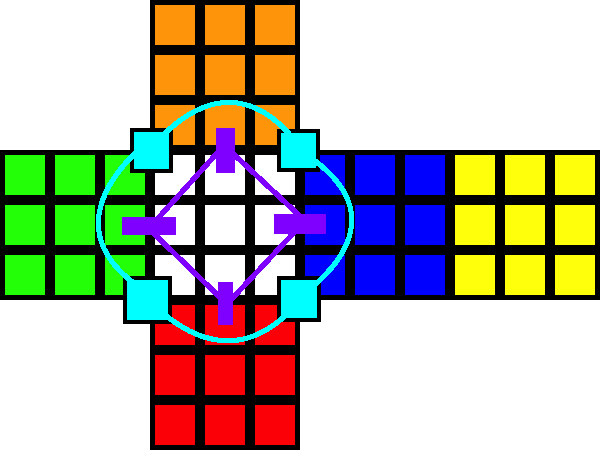
\includegraphics[scale=.5]{images/faceCubieCycle.png} 
\end{center}
We are only concerning ourselves with cycles of the cubies; stickers and orientations will be considered later.  It is clear that this face turn consists of two four-cycles: one of the edge cubies (purple) and one on the corner cubies (cyan).  Since these are cycles of even length, they are odd permutations in the symmetric subgroups concerning the respective cubie permutations.  This means that applying one face turn to the solved cube will bring the cubie permutations out of their respective alternating subgroups, and a second face turn would bring them back.  Thus, any face turn toggles the parity (sign) of \textit{both} symmetric subgroups in tandem.  This means that the symmetric edge and corner components $S_{\text{edges}}, S_{\text{corners}}$ satisfy
\begin{align*}
(S_{\text{edges}},S_{\text{corners}})
&\in
(\mathfrak{A}_{12} \times \mathfrak{A}_7)
\cup
(\bar{\mathfrak{A}_{12}} \times \bar{\mathfrak{A}_7})
\end{align*}
where $\mathfrak{A}_n$ is the alternating group of order.  This is just a restatement of the fact that the parities in the symmetric subgroups must be equal. \\

This means that in a cube state in $O_s$, the edge positions are in an even parity with regards to their symmetric component if and only if the corners are as well, and likewise for odd parities.  Now, consider what happens if we apply a transposition on any two of the edges or corners.  WLOG, assume edges.  That will toggle the edge permutation parity, while preserving the parity of the corner pieces.  There is no legal move to fix this parity error, thus it is a different orbit.  This gives us a factor of 2 in the index $[\mathcal{A}_n : \mathcal{R}_n]$. \\


\end{document}